\begin{question}
\noindent A space observatory uses a tracking grid to record the position of a satellite as it passes overhead. At a certain moment, the satellite is recorded at point $S(2,3)$ on the grid, where the origin $O$ represents the observatory's radar dish.

\begin{center}
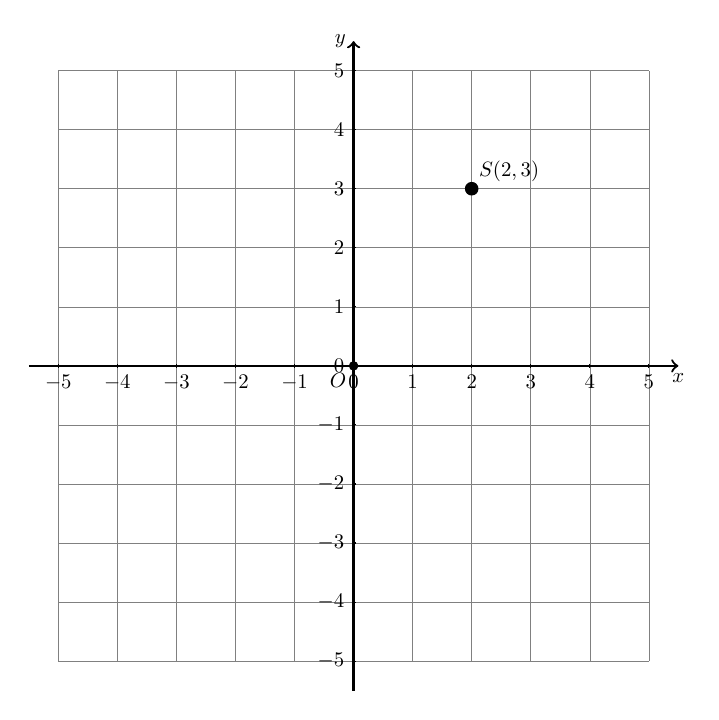
\begin{tikzpicture}[scale=0.75, transform shape]
    \def\axisLimit{5}
    \draw[step=1cm,gray,very thin] (-\axisLimit,-\axisLimit) grid (\axisLimit,\axisLimit);
    \draw[thick,->] (-\axisLimit-0.5,0) -- (\axisLimit+0.5,0) node[anchor=north] {$x$};
    \draw[thick,->] (0,-\axisLimit-0.5) -- (0,\axisLimit+0.5) node[anchor=east] {$y$};
    \foreach \x in {-\axisLimit,...,\axisLimit}
        \draw (\x cm,1pt) -- (\x cm,-1pt) node[anchor=north] {$\x$};
    \foreach \y in {-\axisLimit,...,\axisLimit}
        \draw (1pt,\y cm) -- (-1pt,\y cm) node[anchor=east] {$\y$};

    \filldraw[black] (2,3) circle (3pt) node[above right] {$S(2,3)$};
    \filldraw[black] (0,0) circle (2pt) node[below left] {$O$};
\end{tikzpicture}
\end{center}

\noindent The observatory's software first applies a rotation of $90^\circ$ clockwise about $O$ to correct for Earth's rotation, giving image point $S_1$.

\noindent The software then reflects $S_1$ in the $x$-axis to align with the second dish, giving the final tracked position $S_2$.

\begin{enumerate}
    \item[(a)] Work out the coordinates of $S_1$ and $S_2$.

    \vspace{4cm}
    \answerplain{2}

    \item[(b)] Find the single transformation that maps $S$ directly onto $S_2$.

    \vspace{3cm}
    \answerlines{3}{2}
\end{enumerate}
\end{question}
